\section{Agent-Coordinated Task-Level Operation}
\label{sec:closed-loop-operation}

\begin{figure*}[!t]
\centering
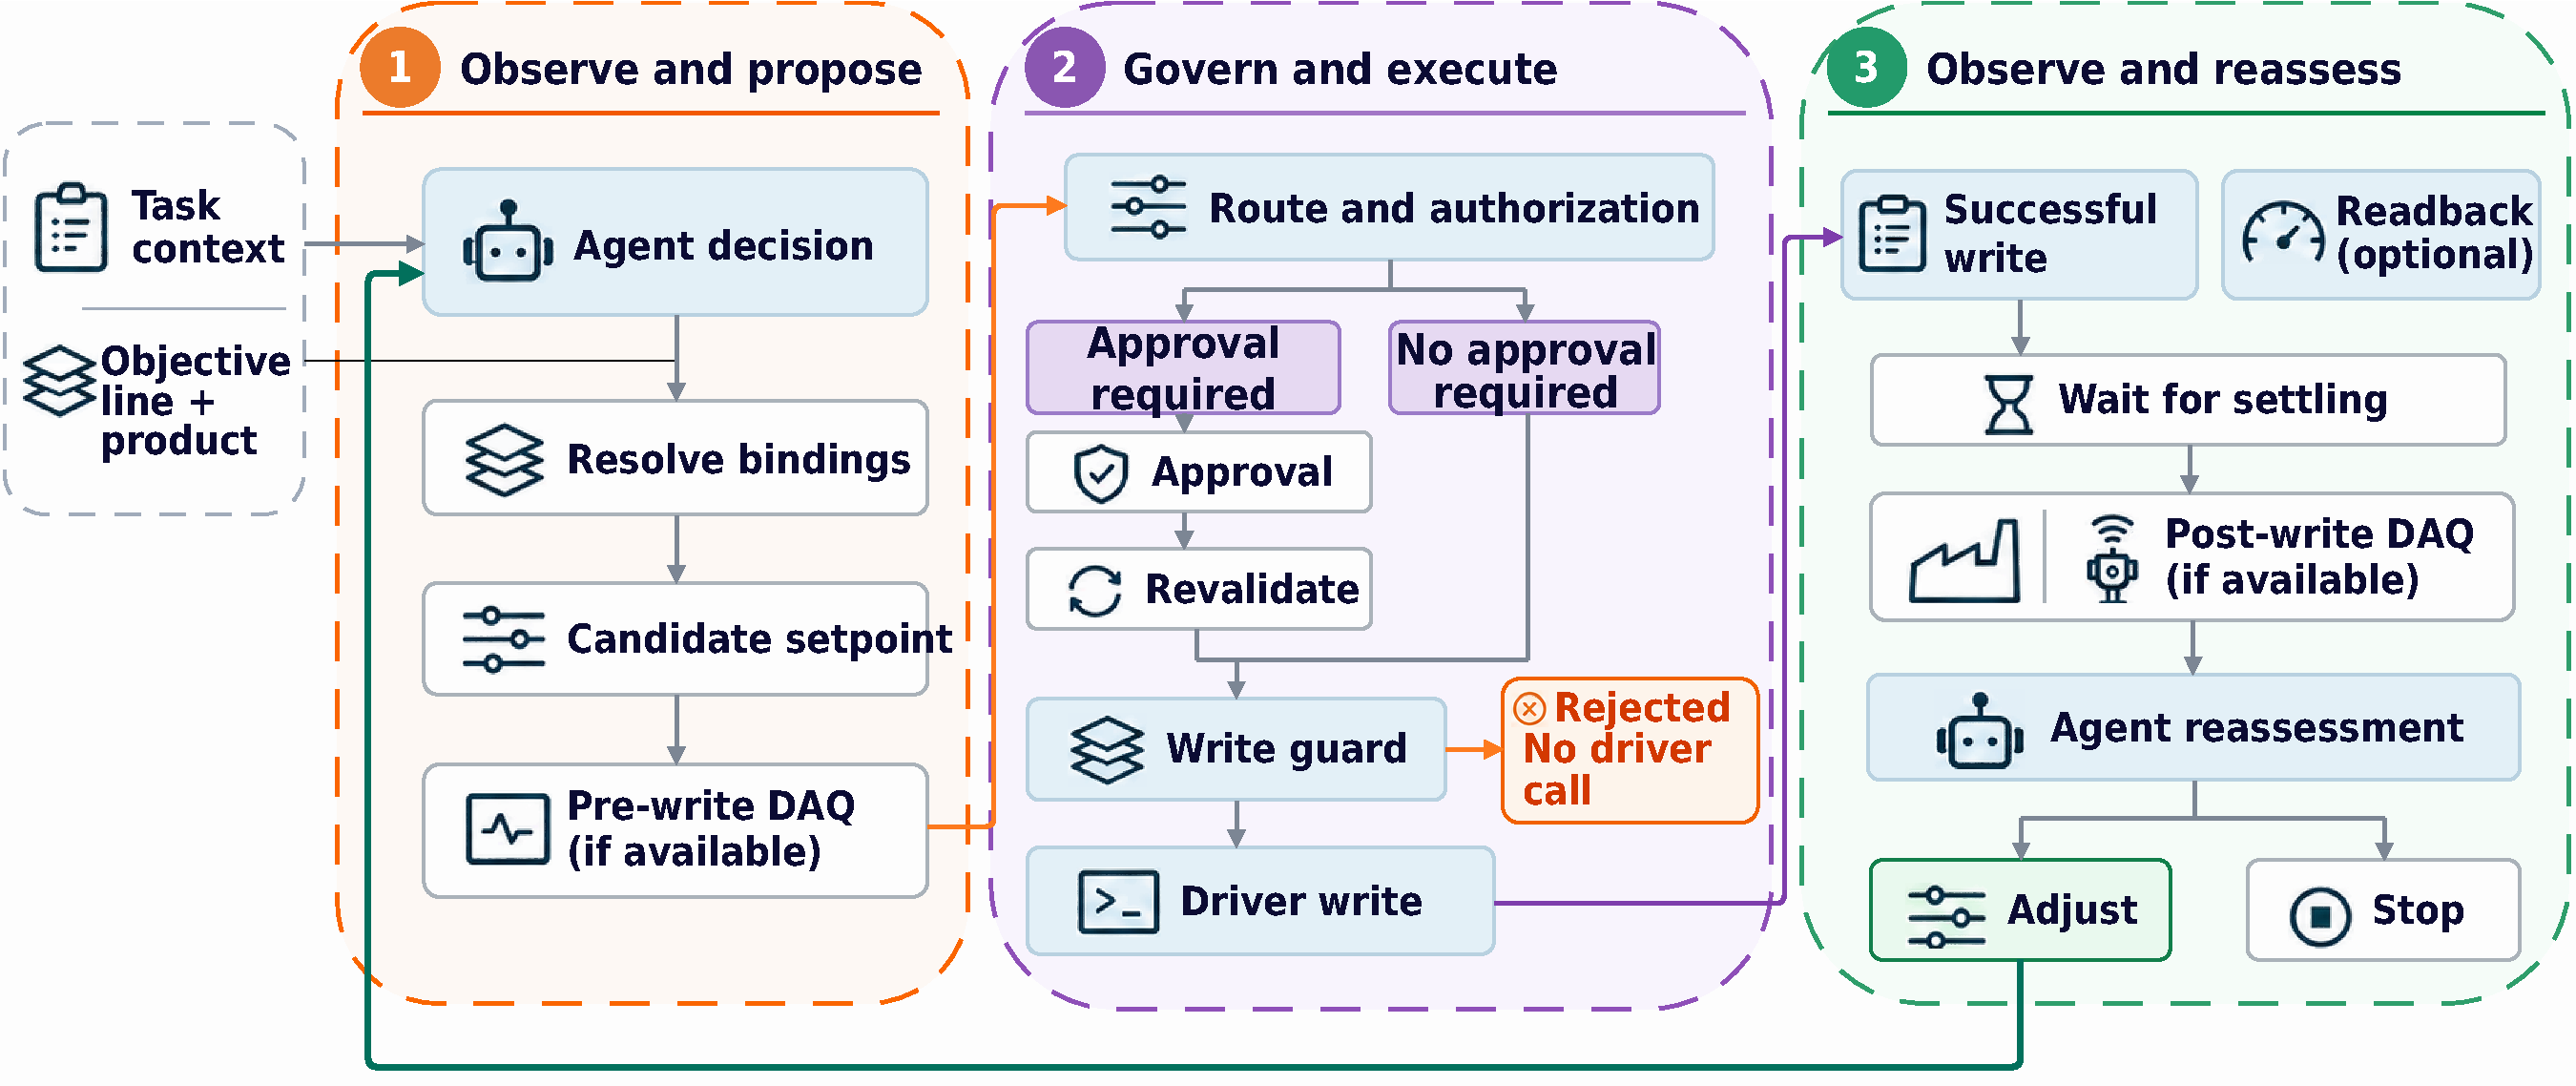
\includegraphics[width=\textwidth]{resources/fig3.pdf}
\caption{Conceptual agent-coordinated optimization loop: an agent proposes a setpoint, the write path applies route-dependent checks, and the agent may reassess available observations before another adjustment or stopping. Requests requiring approval proceed to route-specific revalidation only after approval; requests denied before dispatch do not reach the driver. The approval-denial branch is omitted. Routes without required approval bypass the approval wait but remain subject to applicable dispatch, authorization, and write-guard checks. A driver error may leave device state uncertain. Command outcomes and optional readback are distinct from later DAQ observations; the readback box is schematic.}
\label{fig:agent-loop}
\end{figure*}

A task supplies a process objective and available production context, including the active line, product, and run where present. Fig.~\ref{fig:agent-loop} traces a conceptual iteration from the agent's proposal through governed execution to a later reassessment; it does not depict a successful live-Agent run. Context alone does not authorize a device write. The control node comes from an explicit \texttt{control\_node\_id} or the agent's configured control-write or recipe binding. The DAQ target comes from an explicit ID or agent DAQ binding; a read-only node visible through the channel line is also eligible. Section~\ref{sec:eval} separates scripted process results from exploratory live-Agent episodes.

In goal mode, a lead agent may decompose the objective, dispatch worker subtasks, and assess completion. This optional coordination does not define a control policy. For each step, the responsible agent invokes \texttt{optimization\_explore}, which checks the request before device I/O.

The operation resolves the optimization profile and control-node binding, then uses the node's stored value as the current setpoint $u_0$. This value is not necessarily a fresh device readback. If direction is omitted, the operation defaults to an upward adjustment; otherwise, the supplied direction determines $s\in\{-1,+1\}$. For a step $\Delta u$, it forms
\begin{equation}
 u^{*}=\operatorname{clip}\!\left(u_0+s\Delta u,\,u_{\min},\,u_{\max}\right).
 \label{eq:optimization-candidate}
\end{equation}
In Eq.~(\ref{eq:optimization-candidate}), configured tuning bounds take precedence; node bounds are used otherwise. The effective step is selected in this order: an explicit argument, the binding's tuning step, the scene's maximum step, or one twentieth of the node range.

The operation resolves the DAQ target and checks its visibility. In the later implementation, an optional identifiability preflight blocks a new step if the control node's intervention ledger has an unclosed prior intervention or an unexpired recommended window after an underpowered or confounded verdict. A model--ontology cross-check treats missing evidence as unknown and rejects confirmed conflicts on automatic requests; on the manual path it does not itself block dispatch. Either gate is configurable. If these checks pass, the operation attempts a pre-write DAQ read; its mean may be unavailable. These checks were added after the experiments reported here.

A valid candidate enters the governed single-node write path in Algorithm~1. A pre-dispatch denial stops the request before a driver call. A driver-stage error may occur after dispatch begins, so status alone cannot establish whether the device changed; state must be read and reconciled before retrying.

After a successful write, the operation waits for the configured settling interval (10--300~s; 45~s by default) and attempts a post-write DAQ read. In the later implementation, $t_0$ is recorded before the pre-write read and write call, $\tau$ is the configured wait, and $t_1$ is the time at which the post-write window is requested after that wait. The windows are $[t_0-\tau,t_0]$ and $[t_0,t_1]$. Approval can delay dispatch, so the latter window may include pre-dispatch samples; its mean alone is not causal. The earlier implementation reads trailing 45-s windows. Neither definition establishes causation.

The exploration record retains the control value (the target after a successful write), step, available DAQ means, and write status/message; a rejected attempt has no separate attempted-target field. The shared path separately records command outcome and any device readback. On a later task turn, the agent may review the result, choose another direction and step, or stop. Further iteration requires a subsequent agent decision; the runtime does not autonomously iterate to convergence.


